\section{Problemas Computacionales}

En la sección anterior tratamos con algoritmos para resolver problemas computacionales y estudiamos la corrección y complejidad de esos algoritmos.
Sin embargo se puede estudiar un problema computacional sin ligarse directamente con un algoritmo en particular que lo resuelva, si no más bien ligandose con \emph{todos los posibles algoritmos que lo resuelven}.

Por ejemplo en la sección anterior vinos el algoritmo $\proc{EsPrimo}$ que para un natural $n>2$ verificaba si este era o no divisible por cada uno de los números menores que él y respondía acerca de la \emph{primalidad} (si es o no primo) de $n$.
Vimos también una modificación a este algoritmo que verificaba sólo hasta un umbral de $\sqrt n$ para decidir acerca de la primalidad de $n$.
En ambos casos concluíamos que el algoritmo demoraba tiempo exponencial con respecto a la cantidad de dígitos de $n$ (que era la mejora medida de tamaño del input en este caso).
La pregunta que nos hacemos es >qué tan malo puede ser un algoritmo exponencial en la práctica?
En la siguiente tabla se muestra una estimación del tiempo que le tardaría ejecutar un algoritmo de distintas complejidades en un computador de propósito general.
Estamos suponiendo que el computador puede ejecutar $10^9$ instrucciones por segundo (algo como $1$GHz de velocidad).
\begin{center}
\begin{tabular}{c|cccccccccccccccc}
 & $n=3$ & $n=20$ & $n=100$ & $n=1000$ & $n=10^5$ \\ \hline
$\log n$ & $2\cdot 10^{-9}$ seg & $5\cdot 10^{-9}$ seg & $7\cdot 10^{-9}$ seg & $10^{-8}$ seg& $2\cdot 10^{-8}$ seg \\
$n$ & $3\cdot 10^{-9}$ seg&$2\cdot 10^{-8}$ seg&$10^{-7}$ seg&$10^{-6}$ seg&$10^{-4}$ seg \\
$n^3$&$3\cdot 10^{-8}$ seg&$8\cdot 10^{-6}$ seg&0,001 seg&1 seg&$10$ días \\
$2^n$&$8\cdot 10^{-9}$ seg&0,001 seg&$4\cdot 10^{13}$ años&$3\cdot 10^{284}$ años&$3\cdot 10^{30086} $años\\
$10^n$&$10^{-9}$ seg&$100$ años&$3\cdot 10^{89}$ años&$3\cdot 10^{989}$ años&$\ldots$
\end{tabular}
\end{center}

Vemos que los tiempos exponenciales, incluso para instancias pequeñas (entre 20 y 100) se hacen inmensamente grandes, pero que sin embargo los tiempo polinomiales incluso para instancias grandes se mantienen dentro de lo que se podría estar dispuesto a esperar.
Alguien podría pensar que esperar $10$ días para un algoritmo cúbico ($n^3$) es demasiado, pero este tiempo no es tan grande si pensamos que al contar con un computador que fuese $10$ veces más rápido el tiempo se disminuiría a sólo un día.
Sin embargo para un algoritmo exponencial, no importa que contemos con un computador $10$, $100$ o incluso $10000$ veces más rápido, el tiempo seguirá siendo demasiado alto para instancias pequeñas.
Esto nos da una gran diferencia entre algoritmo polinomiales y exponencial 

Volviendo al problema de determinar si un número es o no primo, conocemos un algoritmo exponencial que lo resuelve >puede hacerse más rápido que eso, o exponencial es lo mejor que podemos lograr?
Esta y otras preguntas motivan las siguientes secciones.

En adelante estaremos más interesados en \emph{problemas de decisión}, o sea, en que las respuestas al problema son SI o NO.
Formalizaremos esta noción en la siguiente sección.

\subsection{%Las Clases de Problemas $P$ y $\NP$ (???)\\ 
Problemas de Decisión y la Clase \emph{P}}

Partiremos definiendo lo que es un \emph{problema de decisión}.
Informalmente un problema de decisión es uno en el cuál las respuestas posibles son SI o NO.
Por ejemplo, si definimos el problema $\proc{PRIMO}$ que se trata de dado un natural $n$ responder SI cuando $n$ sea primo y NO cuando no lo sea, o el problema $\proc{EULERIANO}$ que se trata de dado un grafo conexo $G$ responde SI cuando el grafo contenga un ciclo Euleriano y NO cuando no lo contenga, ambos son problemas de decisión.
Otro ejemplo (muy importante) es el problema $\proc{SAT}$ que se trata de dado una f\'ormula $\varphi$ en l\'ogica proposicional determinar si $\varphi$ es o no satisfacible.


\begin{definicion}
Formalmente un problema de decisión se puede definir en base a pertenencia de elementos a conjuntos.
Un problema de decisión $\pi$ está formado por un conjunto $I_\pi$ de instancias, y un subconjunto $L_\pi$ de él, $L_\pi\subseteq I_\pi$.
El problema $\pi$ se define entonces cómo:
\begin{center}dado un elemento $w\in I_\pi$ determinar si $w\in L_\pi$.\end{center}
Al conjunto $I_\pi$ se le llama conjunto de inputs o de posibles instancias de $\pi$, al conjunto $L_\pi$ se le llama conjunto de  instancias positivas de $\pi$.

Diremos que un algoritmo $A$ resuelve un problema de decisión $\pi$ si para cada input $w\in I_\pi$, el algoritmo $A$ responde SI cuando $w\in L_\pi$ y responde NO cuando $w\in I_\pi-L_\pi$ (para este último caso a veces diremos simplemente $w\notin L_\pi$).
En la figura~\ref{fig:decision} se muestra un diagrama de un problema de decisión y de un algoritmo que lo resuelve.
\begin{figure}[h!]
\centering
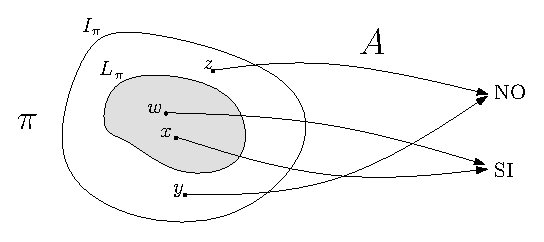
\includegraphics{eps_imgs/decision}
\caption{El algoritmo $A$ resuelve el problema de decisión $\pi$, $w$ y $x$ son instancias positivas del problema (pertenecen a $L_\pi$), $y$ y $z$ no lo son (perteneces a $I_\pi-L_\pi$).}
\label{fig:decision}
\end{figure}
\end{definicion}

\begin{ejemplo}
En el caso del problema de decisión $\proc{PRIMO}$ los conjuntos asociados son $I_{\proc{PRIMO}}=\N-\{0,1\}$ y $L_{\proc{PRIMO}}=\{p\in\N\;|\;p$ es primo$\}$.
El algoritmo $\proc{EsPrimo}$ resuelve el problema $\proc{PRIMO}$ ya que para cada $n\in L_{\proc{PRIMO}}$ responde SI y para cada $n\in I_{\proc{PRIMO}}-L_{\proc{PRIMO}}$ responde NO.

En el caso del problema de decisión $\proc{EULERIANO}$, y suponiendo que $\G$ es el conjunto de todos los grafos, los conjuntos asociados son $I_{\proc{EULERIANO}}=\{G\in\G\;|\; G$ es conexo$\}$ y $L_\proc{EULERIANO}=\{G\in\G\;|\;G$ tiene un ciclo Euleriano$\}$.
El siguiente es un algoritmo para resolver el problema $\proc{EULERIANO}$.
\begin{codebox}
\Procname{INPUT: Un grafo $G$ conexo (asociado a $G$ están los conjuntos $V(G)$ y $E(G)$ de vértices y aristas de $G$). \\
OUTPUT: {\bf SI} si $G$ tiene un ciclo Euleriano, {\bf NO} si no lo tiene.

$\proc{EsEuleriano}(G)$}
\li \For each $v\in V(G)$ \label{li:eseuleriano-for1}
\li \> $\delta:=0$
\li \> \For each $u\in V(G)$ \label{li:eseuleriano-for2}
\li \> \> \If $vu\in E(G)$ \Then
\li \> \> \> $\delta:=\delta+1$
\li \> \If $\delta$ mod $2\not=0$ \Then \label{li:eseuleriano-if}
\li \> \> \Return NO
\li \Return SI
\end{codebox}
El ciclo que comienza en la línea~\ref{li:eseuleriano-for2} cuenta la cantidad de vecinos que tiene un vértice particular $v$ almacenando el resultado en $\delta$, esto lo hace para cada vértice del grafo (ciclo de la línea~\ref{li:eseuleriano-for1}).
Si encuentra algún vértice con una cantidad impar de vecinos entonces responde NO (línea~\ref{li:eseuleriano-if}).
Si todos los vértices tienen una cantidad par de vecinos entonces responde SI.
El algoritmo es correcto por el teorema~\ref{teo:euler}.
La complejidad de este algoritmo es $O(n^2)$ si suponemos que $n=|V(G)|$, osea $n$ es la cantidad de vértices del grafo $G$.
\end{ejemplo}

\begin{ejemplo}
Existen muchos problemas de decisión, algunos de interés teórico, otros de interés más práctico, la siguiente lista presenta otros problemas de decisión.
\begin{itemize}
  \itemsep 0pt
  \item $\proc{CAM-EULER}$: Dado un grafo conexo $G$ determinar si existe un camino Euleriano en él, o sea, un camino no cerrado que contiene a todas las aristas (y todos los vértices) de $G$.
%  En este caso tenemos:
%  \begin{itemize}
%    \itemsep 0pt
%    \item[ ] $I_\proc{CAM-EULER}=\{G\in\G\;|\; G$ es conexo$\}$
%    \item[ ] $L_\proc{CAM-EULER}=\{G\in\G\;|\; G$ tiene un camino Euleriano$\}$
%  \end{itemize}
  \item $\proc{HAMILTONIANO}$: Dado un grafo conexo $G$ determinar si existe un ciclo Hamiltoniano en él, o sea, un ciclo que contiene a todos los vértices de $G$ y que no repite vértices.
%  En este caso tenemos:
%  \begin{itemize}
%    \itemsep 0pt
%    \item[ ] $I_\proc{HAMILTONIANO}=\{G\in\G\;|\; G$ es conexo$\}$
%    \item[ ] $L_\proc{HAMILTONIANO}=\{G\in\G\;|\; G$ tiene un ciclo Hamiltoniano$\}$
%  \end{itemize}
  \item $\proc{CAM-HAMILTON}$: Dado un grafo conexo $G$ determinar si existe un camino Hamiltoniano en él, o sea, un camino no cerrado que contiene a todos los vértices de $G$ y que no repite vértices.
%  En este caso tenemos:
%  \begin{itemize}
%    \itemsep 0pt
%    \item[ ] $I_\proc{CAM-HAMILTON}=\{G\in\G\;|\; G$ es conexo$\}$
%    \item[ ] $L_\proc{CAM-HAMILTON}=\{G\in\G\;|\; G$ tiene un camino Hamiltoniano$\}$
%  \end{itemize}
  \item $\proc{CLIQUE}$: Dado un grafo $G$ y un natural $k$ determinar si $G$ tiene un clique de tamaño $k$ (clique con $k$ vértices).
  \item $\proc{INDEPENDIENTE}$: Dado un grafo $G$ y un natural $k$ determinar si $G$ tiene un conjunto independiente de tamaño $k$ (clique con $k$ vértices).
  \item $\proc{BIPARTITO}$: Dado un grafo $G$ determinar si $G$ es un grafo bipartito.
  \item $\proc{COMPILA-C}$: Dado un string $s$ de caracteres ASCII determinar si $s$ es un programa correctamente escrito según la sintaxis de C.
  \item $\proc{OCURRENCIA}$: Dado un par de strings $s_1$ y $s_2$ de caracteres ASCII determinar si $s_2$ ocurre como sub--string de $s_1$.
  \item $\proc{ORDEN}$: Dada una secuencia de enteros $S=(s_1,s_2,\ldots,s_n)$ decidir si la secuencia se encuentra ordenada.
  \item $\proc{MIN}$: Dado un número entero $m$ y una secuencia de enteros $S=(s_1,s_2,\ldots,s_n)$, determinar si $m$ es el mínimo de la secuencia $S$.
  \item $\proc{MCD}:$ Dado un trío de naturales $l,m$ y $n$ determinar si $n$ es el máximo común divisor de $m$ y $l$.
  \item $\proc{COMPUESTO}$: Dado un número natural $n$ determinar si $n$ es un número compuesto (o sea si $n$ no es un número primo).
\end{itemize}
Como ejercicio, para cada uno de estos problemas se puede encontrar sus conjuntos $I_\pi$ y $L_\pi$ asociados.
\end{ejemplo}

En el ejemplo anterior, el problema de decisión $\proc{MCD}$ proviene del problema de búsqueda ``dados dos naturales $l$ y $m$, encontrar el máximo común divisor entre ellos'', algo similar ocurre con los problemas $\proc{ORDEN}$ y $\proc{MIN}$.
%El problema de decisión $k\proc{-CLIQUE}$ por su parte, proviene del problema de optimización ``dado un grafo $G$ determinar la cantidad de vértices que tiene el clique de tamaño máximo en $G$''.
%En el ejemplo $\proc{MCD}$ vemos cómo se transformó el problema de búsqueda ``dados dos naturales $l$ y $m$, encontrar el máximo común divisor'', en el problema de decisión ``decidir si $n$ es el máximo común divisor de $l$ y $m$''.
%Por su parte, en el ejemplo del problema $\proc{CLIQUE}$ vemos cómo se transformó el problema de optimización ``dado un grafo $G$ determinar el tamaño del clique máximo'' en el problema de decisión ``decidir si el clique de tamaño máximo en $G$ tiene tamaño $k$''.
La mayoría de los problemas de búsqueda (o incluso de optimización) se pueden transformar de manera similar en problemas de decisión.

Estamos interesados en clasificar los problemas según su dificultad \emph{en la práctica}, en cuanto a qué tan rápido puede ser un algoritmo que lo resuelva.
Ya dimos evidencia de que un algoritmo exponencial es impracticable, pero que un algoritmo polinomial parecía ser mucho más realizable.
Para formalizar estas nociones intuitivas usaremos las siguientes definiciones.

\begin{definicion}
Definimos el conjunto $P$ de todos los problemas de decisión $\pi$ para los cuales existe un algoritmo de complejidad a lo más polinomial en el peor caso que resuelve $\pi$
\[
P=\{\pi\text{ problema de decisión}\;|\;\text{existe un algoritmo de peor caso polinomial para resolver }\pi\}
\]
O sea, $\pi\in P$ si existe un natural $k$ y un algoritmo $A$ que resuelve $\pi$, tal que $A$ es de complejidad $O(n^k)$ en el peor caso si $n$ es el tamaño de la instancia para $A$.
Diremos (informalmente) que un problema $\pi$ es \emph{tratable} o \emph{soluble eficientemente en la práctica} si $\pi\in P$.
\end{definicion}


El algoritmo $\proc{EsEuleriano}$ resuelve el problema $\proc{EULERIANO}$ en tiempo $O(n^2)$ en el peor caso, por lo que $\proc{EULERIANO}\in P$.
No es difícil argumentar (ejercicio) que los siguientes problemas también están en $P$: $\proc{CAM-EULER}$, $\proc{OCURRENCIA}$, $\proc{ORDEN}$, $\proc{MIN}$, $\proc{MCD}$.
Tal vez no podemos dar una argumentación formal acerca de que el problema $\proc{COMPILA-C}$ pertenece a $P$, sin embargo la noción intuitiva de $P$ nos ayuda en este caso, de hecho, 
todos los días hay gente compilando programas en C y en ningún caso ocurre que un programa demore años en compilar, dado que es un problema que se resuelve continuamente en la práctica este debe estar en $P$, de hecho efectivamente ocurre que $\proc{COMPILA-C}\in P$.

Un caso a parte lo tiene el problema $\proc{PRIMO}$.
Hemos mostrado un algoritmo ($\proc{EsPrimo}$) que resuelve el problema pero que tarda tiempo exponencial $O(3^d)$ (el algoritmo mejorado) con $d$ la cantidad de dígitos del número de input.
Este hecho no nos permite concluir nada acerca de si $\proc{PRIMO}$ pertenece o no a $P$, de hecho no nos entrega información alguna.
Hasta el año 2002 no se sabía si el problema $\proc{PRIMO}$ estaba o no en $P$ y la pregunta acerca de si existía un algoritmo eficiente para determinar si un número era primo había estado abierta durante siglos.
En 2002, Agrawal, Kayal y Saxena (todos científicos Indios) encontraron un algoritmo de peor caso polinomial para resolver el problema $\proc{PRIMO}$ y por lo tanto ahora sabemos que $\proc{PRIMO}\in P$.
Una conclusión directa es que $\proc{COMPUESTO}\in P$ también.

>Existen problemas que se sepa que no están en $P$?
La respuesta es SI, existen de hecho problemas para los cuales ni siquiera existe un algoritmo (de ninguna complejidad!) que los resuelva, pero esta discusión está fuera del alcance de nuestro estudio.

Nos interesan otro tipo de problemas que no se saben si están o no en $P$ pero cuya respuesta traería implicaciones importantísimas en el área de computación.

\begin{ejemplo}[Coloración de Mapas.]
Una coloración de un mapa en un plano, es una asignación de colores para cada país en el mapa, tal que a dos países vecinos se les asigna colores diferentes.
Países vecinos son los que comparten alguna frontera.
Para simplificar supondremos que los colores son números naturales.
En la figura~\ref{fig:map1} se muestra un mapa y una posible coloración para él.
\begin{figure}[h!]
\vspace*{200pt}
\caption{}
\label{fig:map1}
\end{figure}
La coloración tiene 5 colores, una pregunta válida es >podremos colorearlo con menos de 5 colores?
La respuesta es SI, de hecho sólo 4 son necesarios.

En 1977 Appel y Haken demostraron que cualquier mapa puede ser coloreado con 4 colores, sólo 4 colores son suficientes.
Este hecho había sido una conjetura durante más de 100 años, se propuso inicialmente en el año 1853.
La demostración de Appel y Haken se basó en el uso intensivo de poder computacional (ver \verb|http://mathworld.wolfram.com/Four-ColorTheorem.html| para más información).

Nos podemos plantear el problema de decisión $4\proc{-MAP-COLOR}$ que dado un mapa en el plano decide si este puede o no pintarse con 4 colores.
El resultado de Appel y Haken nos permite hacer un algoritmo trivial para resolver este problema, uno que responde siempre SI para toda instancia.

Dado que la solución al problema anterior resulta trivial, nos podemos plantear los siguientes problemas no triviales:
\begin{itemize}
  \itemsep 0pt
  \item $2\proc{-MAP-COLOR}$: Dado un mapa en el plano decidir si este puede pintarse con sólo 2 colores.
  \item $3\proc{-MAP-COLOR}$: Dado un mapa en el plano decidir si este puede pintarse con sólo 3 colores.
\end{itemize}
Lo primero es notar que cualquier instancia positiva de $2\proc{-MAP-COLOR}$ es también una instancia positiva de $3\proc{-MAP-COLOR}$, pero no a la inversa.
Lo otro que se puede decir es que para resolver el problema $2\proc{-MAP-COLOR}$ existe un algoritmo que toma tiempo polinomial en la cantidad de países del mapa y que por lo tanto $2\proc{-MAP-COLOR}\in P$....

>Qué pasa con el problema $3\proc{-MAP-COLOR}$?
En lo que sigue diseñaremos un algoritmo que lo resuelve.
Dado un mapa con $n$ países, numeraremos sus países de $1$ a $n$, y representaremos el mapa por una matriz de adyacencia $M$ tal que $M_{ij}=1$ si los países $i$ y $j$ son vecinos, $0$ en otro caso.
Una asignación de colores para $M$ la modelaremos como una secuencia $C=(c_1,c_2,\ldots,c_n)$ donde $c_i$ es el color asignado al país $i$ y cada $c_i\in\{0,1,2\}$.
Note que a cada secuencia $C$ distinta le corresponde un único número en base $3$ entre $0$ y $3^n-1$, entonces podemos usar un procedimiento similar al algoritmo $\proc{Base3}$ de la sección anterior para generar sistemáticamente las coloraciones posibles.
El siguiente algoritmo $\proc{3-Coloracion}$ resuelve el problema $3\proc{-MAP-COLOR}$, usa un procedimiento auxiliar $\proc{Verifica-Coloracion}$.
\begin{codebox}
\Procname{
INPUT: Una matriz $M$ representante de un mapa en el plano y la cantidad de países $n$. \\
OUTPUT: {\bf SI} si el mapa representado por $M$ puede ser coloreado con $3$ colores, {\bf NO} si se necesitan más de $3$ colores para colorear $M$.

$\proc{3-Coloracion}(M,n)$}
\li \For $i:=0$ \To $3^n-1$
\li \> $C=\proc{Base3}(i)$
\li \> \If $\proc{Verifica-Coloracion}(M,n,C)$ \Then
\li \> \> \Return SI
\li \Return NO
\end{codebox}
\begin{codebox}
\Procname{$\proc{Verifica-Coloracion}(M,n,C)$}
\li \For $i:=1$ \To $n-1$
\li \> \For $j:=i+1$ \To $n$
\li \> \> \If $M_{ij}=1\;\wedge\;c_i=c_j$ \Then
\li \> \> \> \Return {\bf false}
\li \Return {\bf true}
\end{codebox}
El algoritmo $\proc{3-Coloracion}$ hace en el peor caso $3^n$ llamadas al procedimiento $\proc{Verifica-Coloracion}$ y dado que este último procedimiento toma tiempo $\Theta(n^2)$ con $n$ la cantidad de países, $\proc{3-Coloracion}$ toma tiempo $\Theta(3^{n^2})$ en el peor caso.
Este algoritmo claramente no es polinomial, esto no indica que $\proc{3-MAP-COLOR}$ no pertenezca a $P$, sólo nos dice que probando todas las posibilidades no obtenemos resultados realizables en la práctica.
>Hay alguna manera polinomial de resolver el problema?
Hasta el día de hoy no se ha encontrado un algoritmo polinomial para resolverlo, a grandes razgos lo mejor que se puede hacer es probar todas las posibilidades...
\end{ejemplo}

Hay muchos problemas de decisión de importancia práctica y teórica que están en la misma situación que $\proc{3-MAP-COLOR}$, estudiaremos estos problemas en la siguiente sección.

\subsection{La Clase $\NP$ y Problemas $\NP$-completos}

En esta sección analizaremos una generalización del concepto de que un problema sea \emph{tratable} o \emph{soluble eficientemente en la práctica}.
Antes dijimos que un problema $\pi$ es \emph{tratable} si ocurre que $\pi\in P$, o sea, si existe un algoritmo para resolver $\pi$ que toma tiempo polinomial en el peor caso.
Esta definición deja en \emph{el limbo} a problemas como $\proc{3-MAP-COLOR}$ para los cuales aun no se sabe si existe o no un algoritmo polinomial que lo resuelva.
Para abarcar a este tipo de problemas se define la clase $\NP$ de problemas computacionales.

Existe una noción intuitiva simple de entender y muy útil para determinar cuándo un problema está en la clase de problemas $\NP$.
Suponga que hay dos personas $A$ y $V$ analizando el problema de decisión $\pi$, y supongamos que la persona $A$ de alguna manera determina que una instancia posible $w\in I_\pi$ es una instancia positiva para $\pi$, o sea $w\in L_\pi$, entonces $A$ siempre podrá encontrar ``una forma de convencer rápidamente'' a $V$ de que $w$ efectivamente es una instancia positiva para $\pi$.
La frase ``una forma de convencer rápidamente'' es bastante imprecisa, con ``una forma'' nos referimos a algún tipo de información asociada a $w$ que sirva para que convencer a $V$, y con ``convencer rápidamente'' nos referimos a que $V$ puede verificar en tiempo a lo más polinomial (ayudado con la información proporcionada por $A$) que $w$ es una instancia positiva.
Por ejemplo, en el problema $\proc{3-MAP-COLOR}$ si dado un mapa $M$, $A$ determina que $M$ puede ser coloreado con tres colores, basta con que $A$ le muestre a $V$ una asignación válida de colores para que $V$ en tiempo polinomial se convenza de que efectivamente $M$ era una instancia positiva, lo único que debería hacer $V$ es verificar que la asignación mostrada por $A$ no produce conflictos en los países de $M$.
A la persona $A$ se le llama \emph{adivinador} y a la persona $V$ se le llama \emph{verificador}.
Entonces, Un problema $\pi\in\NP$ si para cada $w\in L_\pi$, el \emph{adivinador} puede convencer en tiempo polinomial al \emph{verificador} de que efectivamente $w\in L_\pi$.

La noción de ``adivinar'' y ``verificar'' se ve claramente en el algoritmo desarrollado para $\proc{3-MAP-COLOR}$ de la sección anterior.
En el procedimiento $\proc{3-Coloracion}$, en el ciclo de la línea 1, se está tratando de encontrar una secuencia de colores que formen una coloración válida para el mapa $M$ de input. 
Si $M$ efectivamente se puede colorear con tres colores, estamos seguros de que el ciclo encontrará una secuencia de colores válida.
Por su parte el procedimiento $\proc{Verifica-Coloracion}$ es el encargado de verificar que una asignación de colores encontrada es efectivamente una coloración válida.
El ciclo principal en $\proc{3-Coloracion}$ está ``adivinando'', el procedimiento $\proc{Verifica-Coloracion}$ por su parte está ``verificando'', verificación que se lleva a cabo en tiempo polinomial con respecto al tamaño del input (tiempo $\Theta(n^2)$ si $n$ es la cantidad de países).

\begin{ejemplo}
Ya vimos que $\proc{3-MAP-COLOR}\in\NP$ ya que para cada mapa que puede colorearse con tres colores, basta con que el \emph{adivinador} le muestre la asignación de colores al \emph{verificador} para que este se convenza en tiempo polinomial de que el mapa efectivamente se podía colorear con tres colores.

También ocurre que $\proc{HAMILTONIANO}\in\NP$, ya que si un grafo $G$ es efectivamente Hamiltoniano, basta con que el \emph{adivinador} le muestre al \emph{verificador} un ciclo en $G$ que pasa por todos los vértices para que este último se convenza en tiempo polinomial de que $G$ efectivamente era Hamiltoniano.

No es difícil darse cuenta que todos los problemas en la lista de problemas de decisión de la sección anterior pertenecen también a $\NP$.
Mención especial se podría hacer por ejemplo con el problema $\proc{MIN}$, >de qué forma convence el \emph{adivinador} al \emph{verificador} de que dado un valor $m$ y una secuencia de valores $S=(s_1,s_2,\ldots,s_n)$, $m$ es el mínimo de la secuencia $S$?
En este caso resulta que el \emph{adivinador} no tiene que hacer nada, el \emph{verificador} puede ``convencerse sólo'' ya que dado que $\proc{MIN}\in P$, el \emph{verificador} en tiempo polinomial puede comprobar que efectivamente $m$ es el mínimo de $S$.
%Algo similar ocurre con los problemas $\proc{EULERIANO},\proc{ORDEN},\proc{OCURRENCIA}$ etc.
\end{ejemplo}

Este último ejemplo nos permite deducir lo siguiente: si un problema $\pi\in P$ entonces necesariamente $\pi\in\NP$ ya que, dado que para $\pi$ existe un algoritmo polinomial, el \emph{verificador} puede ``convencerse sólo'' en tiempo polinomial de que una instancia $w$ efectivamente está en $L_\pi$, no necesita ayuda del \emph{adivinador}.

Formalizaremos la noción hasta ahora intuitiva de $\NP$ en la siguiente definición.

\begin{definicion}
Un problema de decisión $\pi$ pertenece a la clase de problemas $\NP$ si 
existe un algoritmo $V$ y una funci\'on $c$ definida sobre $L_\pi$ tal que
para cada instancia $w\in L_\pi$:
\begin{itemize}
\item $c(w)$ es de tamaño polinomial con respecto a $w$, y 
\item el algoritmo $V$ con input $w$ y $c(w)$ responde SI en tiempo polinomial (con respecto a $w$).
\end{itemize}
Es decir, usando el \emph{certificado} $c(w)$ el algoritmo $V$ verifica
en tiempo polinomial que $w$ efectivamente pertenece a $L_\pi$.
\end{definicion}

\begin{ejemplo}
En el caso del problema $\proc{3-MAP-COLOR}$, dado un mapa $M$ que se puede colorear con tres colores, el certificado $c(M)$ es la asignación de colores válida para $M$.
El algoritmo $\proc{Verifica-Asignacion}$ usando $c(M)$ verifica en tiempo polinomial que $M$ efectivamente se puede colorear con tres colores.

Para el problema $\proc{HAMILTONIANO}$, dado un grafo Hamiltoniano $G$, el certificado $c(G)$ es una permutación de los vértices de $G$ que formen un ciclo en $G$.
En tiempo polinomial se puede chequear que $c(G)$ es efectivamente un ciclo en $G$ que contiene a todos los vértices y por lo tanto que $G$ es Hamiltoniano.

Para el problema $\proc{BIPARTITO}$, dado un grafo bipartito $G$, el certificado $c(G)$ es el par de conjunto $(V,U)$ que conforman la bipartición de $G$.
Dados los conjuntos $V$ y $U$ se puede chequear en tiempo polinomial que $G$ es bipartito, basta verificar que tanto $V$ como $U$ son conjuntos independientes en $G$.

Para el problema $\proc{CLIQUE}$, dado un grafo $G$ que posee un clique de tamaño $k$, el certificado $c(G)$ es un subconjunto $K$ de vértices de $G$ tal que $|K|=k$ y todos los vértices de $K$ son vecinos mutuos.
Dado $K$, se puede en tiempo polinomial verificar que su tamaño es $k$ y que todos sus vértices son vecinos mutuos en $G$.

Para el problema $\proc{EULERIANO}$, dado un grafo Euleriano $G$, el certificado sería simplemente el mismo $G$ ya que en tiempo polinomial se puede verificar que $G$ es Euleriano mirando los grados de cada uno de sus vértices.
\end{ejemplo}

Este último ejemplo nos indica cómo los problemas en $P$ son siempre un caso particular de los problemas en $\NP$.
%A partir de la definición de la clase de problemas $\NP$ se podría definir la clase de problemas $P$ como el subconjunto de $\NP$ de todos los problemas para los cuales el certificado $c(w)$ para una instancia positiva es la misma instancia $w$.
Podemos, a partir de la definición de la clase de problemas $\NP$, definir la clase de problemas $P$, como un subconjunto de $\NP$, de la siguiente forma: En $P$ están todos los problemas $\pi$ de $\NP$ tales que el certificado asociado a cada instancia positiva $w$ de $\pi$ es la misma instancia $w$, o sea, tales que $\forall w\in L_\pi$ $c(w)=w$.
De esta última discusión %más otras anteriores nos hacen concluir que todo problema que pertenece a la clase $P$ pertenece también en la clase $\NP$, de donde 
obtenemos que 
\[
P\subseteq \NP.
\]
Sin embargo existen problemas en $\NP$ para los cuales no se sabe si hay una solución en tiempo polinomial como $\proc{3-MAP-COLOR}$ por ejemplo, luego las siguientes son preguntas válidas
\[
\text{¿ }P=\NP\text{ ?}\;\;\;\;\;\;\;\;\;\;\;\;\text{¿ }P\not=\NP\text{ ?}
\]
Si la primera de estas preguntas fuera cierta entonces sabríamos que todo problema en $\NP$ tendría una solución polinomial y entonces existiría un algoritmo polinomial para el problema $\proc{3-MAP-COLOR}$.
Si en cambio la segunda de estas preguntas fuera cierta, entonces existiría {\bf al menos un problema} en $\NP$ para el cual {\bf no hay algoritmo polinomial} que lo resuelva.
Veremos que si este último es el caso entonces existirían muchos problemas para los cuales no se podría encontrar un algoritmo polinomial que lo resuelva.

La pregunta acerca de si $P=NP$ o $P\not=NP$ es una de las preguntas abiertas más importantes (si no la más importante) en ciencia de la computación, y desde el momento en que se propuso en el año 1971, hasta la fecha no parece haber un avance significativo para poder responderla.
Sin embargo, existe mucha más evidencia acerca de que $P\not=NP$ principalmente por la existencia de los llamados problemas $\NP$-completos.
Intuitivamente un problema $\NP$-completo es un problema que es {\bf más difícil que todos} los problemas en $\NP$, en el sentido de que si se pudiera resolver en tiempo polinomial, entonces todos los problemas de $\NP$ se podrían resolver también en tiempo polinomial.

\begin{definicion}
Un problema de decisión $\pi$ es $\NP$-completo si $\pi\in\NP$ y, si existiera un algoritmo polinomial para resolver $\pi$, entonces se podría encontrar a partir del algoritmo para $\pi$ un algoritmo polinomial para resolver cada uno de los problemas en $\NP$.
\end{definicion}

\begin{teorema}[(Cook)]
$\proc{SAT}$ es NP-completo. M\'as aun, $\proc{3-CNF-SAT}$ (o sea $\proc{SAT}$ para f\'ormulas en CNF donde cada 
cl\'ausula tiene 3 literales) es NP-completo.
\end{teorema}

\begin{teorema}
El problema $\proc{3-COLOR}$ es $\NP$-completo,
el problema $\proc{HAMILTONIANO}$ es $\NP$-completo,
el problema $\proc{INDEPENDIENTE}$ es $\NP$-completo,
el problema $\proc{CLIQUE}$ es $\NP$-completo.
\end{teorema}

Muchos otros problemas de decisión de interés práctico y teórico son tambi\'en $\NP$-completos.
Hasta la fecha siguen apareciendo nuevos problemas en las más diversas áreas que caen también dentro de esta categoría.
La implicación más importante de que un problema sea $\NP$-completo es que si se llegara a encontrar un algoritmo polinomial para él, entonces se podría encontrar una solución polinomial para todos los problemas en $\NP$.
Por ejemplo, si alguien encontrara un algoritmo polinomial para resolver el problema $\proc{3-COLOR}$ entonces inmediatamente se podría encontrar un algoritmo polinomial para $\proc{HAMILTONIANO}$, $\proc{CLIQUE}$, y todos los otros problemas $\NP$-completos.

%\subsection{Reducción de Problemas y Demostraciones de \emph{NP}-completitud**}
%[...falta completar...]

%\subsection{Otras Clases de Problemas Computacionales**}
%[...falta completar...]
